\documentclass[UTF8]{ctexart}
\usepackage{geometry, CJKutf8, graphicx}
\geometry{margin=1.5cm, vmargin={0pt,1cm}}
\setlength{\topmargin}{-1cm}
\setlength{\paperheight}{29.7cm}
\setlength{\textheight}{25.3cm}

% useful packages.
\usepackage{amsfonts}
\usepackage{amsmath}
\usepackage{amssymb}
\usepackage{amsthm}
\usepackage{enumerate}
\usepackage{graphicx}
\usepackage{multicol}
\usepackage{fancyhdr}
\usepackage{layout}
\usepackage{listings}
\usepackage{float, caption}

\lstset{
    basicstyle=\ttfamily, basewidth=0.5em
}

% some common command
\newcommand{\dif}{\mathrm{d}}
\newcommand{\avg}[1]{\left\langle #1 \right\rangle}
\newcommand{\difFrac}[2]{\frac{\dif #1}{\dif #2}}
\newcommand{\pdfFrac}[2]{\frac{\partial #1}{\partial #2}}
\newcommand{\OFL}{\mathrm{OFL}}
\newcommand{\UFL}{\mathrm{UFL}}
\newcommand{\fl}{\mathrm{fl}}
\newcommand{\op}{\odot}
\newcommand{\Eabs}{E_{\mathrm{abs}}}
\newcommand{\Erel}{E_{\mathrm{rel}}}

\begin{document}

\pagestyle{fancy}
\fancyhead{}
\lhead{马竞轩, 3230103014}
\chead{数据结构与算法第五次作业}
\rhead{Nov.4th, 2024}

\section{detachMin()函数}
\subsection{功能}
查找以t为根的子树中的最小节点,返回这个节点,并从原子树中删除这个节点。
\subsection{参数}
指向一个子树root的指针,并且为引用,因此函数内部修改t时,直接修改实参。
\subsection{返回值}
指向被删除(子树中的最小节点)的节点的指针。
\subsection{功能实现}
一共分两种情况。
\begin{enumerate}
\item t所指的子树只有一个根,或根只有右节点:

此时最小节点就是根。指向t的指针修改为指向\lstinline{t->right}即可。
\item t所指的根有左节点:

不断向左节点寻找子树中的最小节点,最终得到指向最小节点的指针,此时删除这个最小节点就是remove()中“只有一个孩子”的情况,只需简单修改指针指向即可。
\end{enumerate}
注:根据remove()中调用detachMin()的逻辑,t一定不会是空树。

\section{remove()函数}
\subsection{功能}
删除指定节点。若找不到该节点,则输出错误提示。
\subsection{参数}
外部:要删除的节点内容。
内部:要删除的节点内容,以及指向当前节点的指针t。同样t为引用,修改实参。
\subsection{返回值}
无
\subsection{功能实现}
先执行寻找过程,若要找的节点小于当前节点,则向左节点寻找,反之向右节点寻找。若最终当前节点为nullptr,则说明找不到该节点,输出错误提示。若此时找到了该节点,则分多种情况讨论。设此时t指向的节点为currentNode,注意此时t为currentNode的父节点指向currentNode的指针,由于t是引用,修改t直接修改父节点的left或right的指针。
\begin{enumerate}
\item 要删除的节点只有一个孩子,或没有孩子:

指向currentNode的节点改为指向currentNode的孩子,然后删除currentNode。
\item 要删除的节点有两个孩子:

使用detachMin()函数找到currentNode右节点的最小节点,使它从树中脱离出来,通过修改若干指针的方法替换currentNode位置,再将currentNode删除。
\end{enumerate}
\section{测试结果与分析}
有几个要点需要考虑:要删除的元素是否找得到?currentNode是否为根节点?currentNode有几个孩子?currentNode的右节点有几个孩子?据此设计测试程序(详细测试方案见输出内容),最后再进行空树的异常测试。

附上测试对应的分析图:

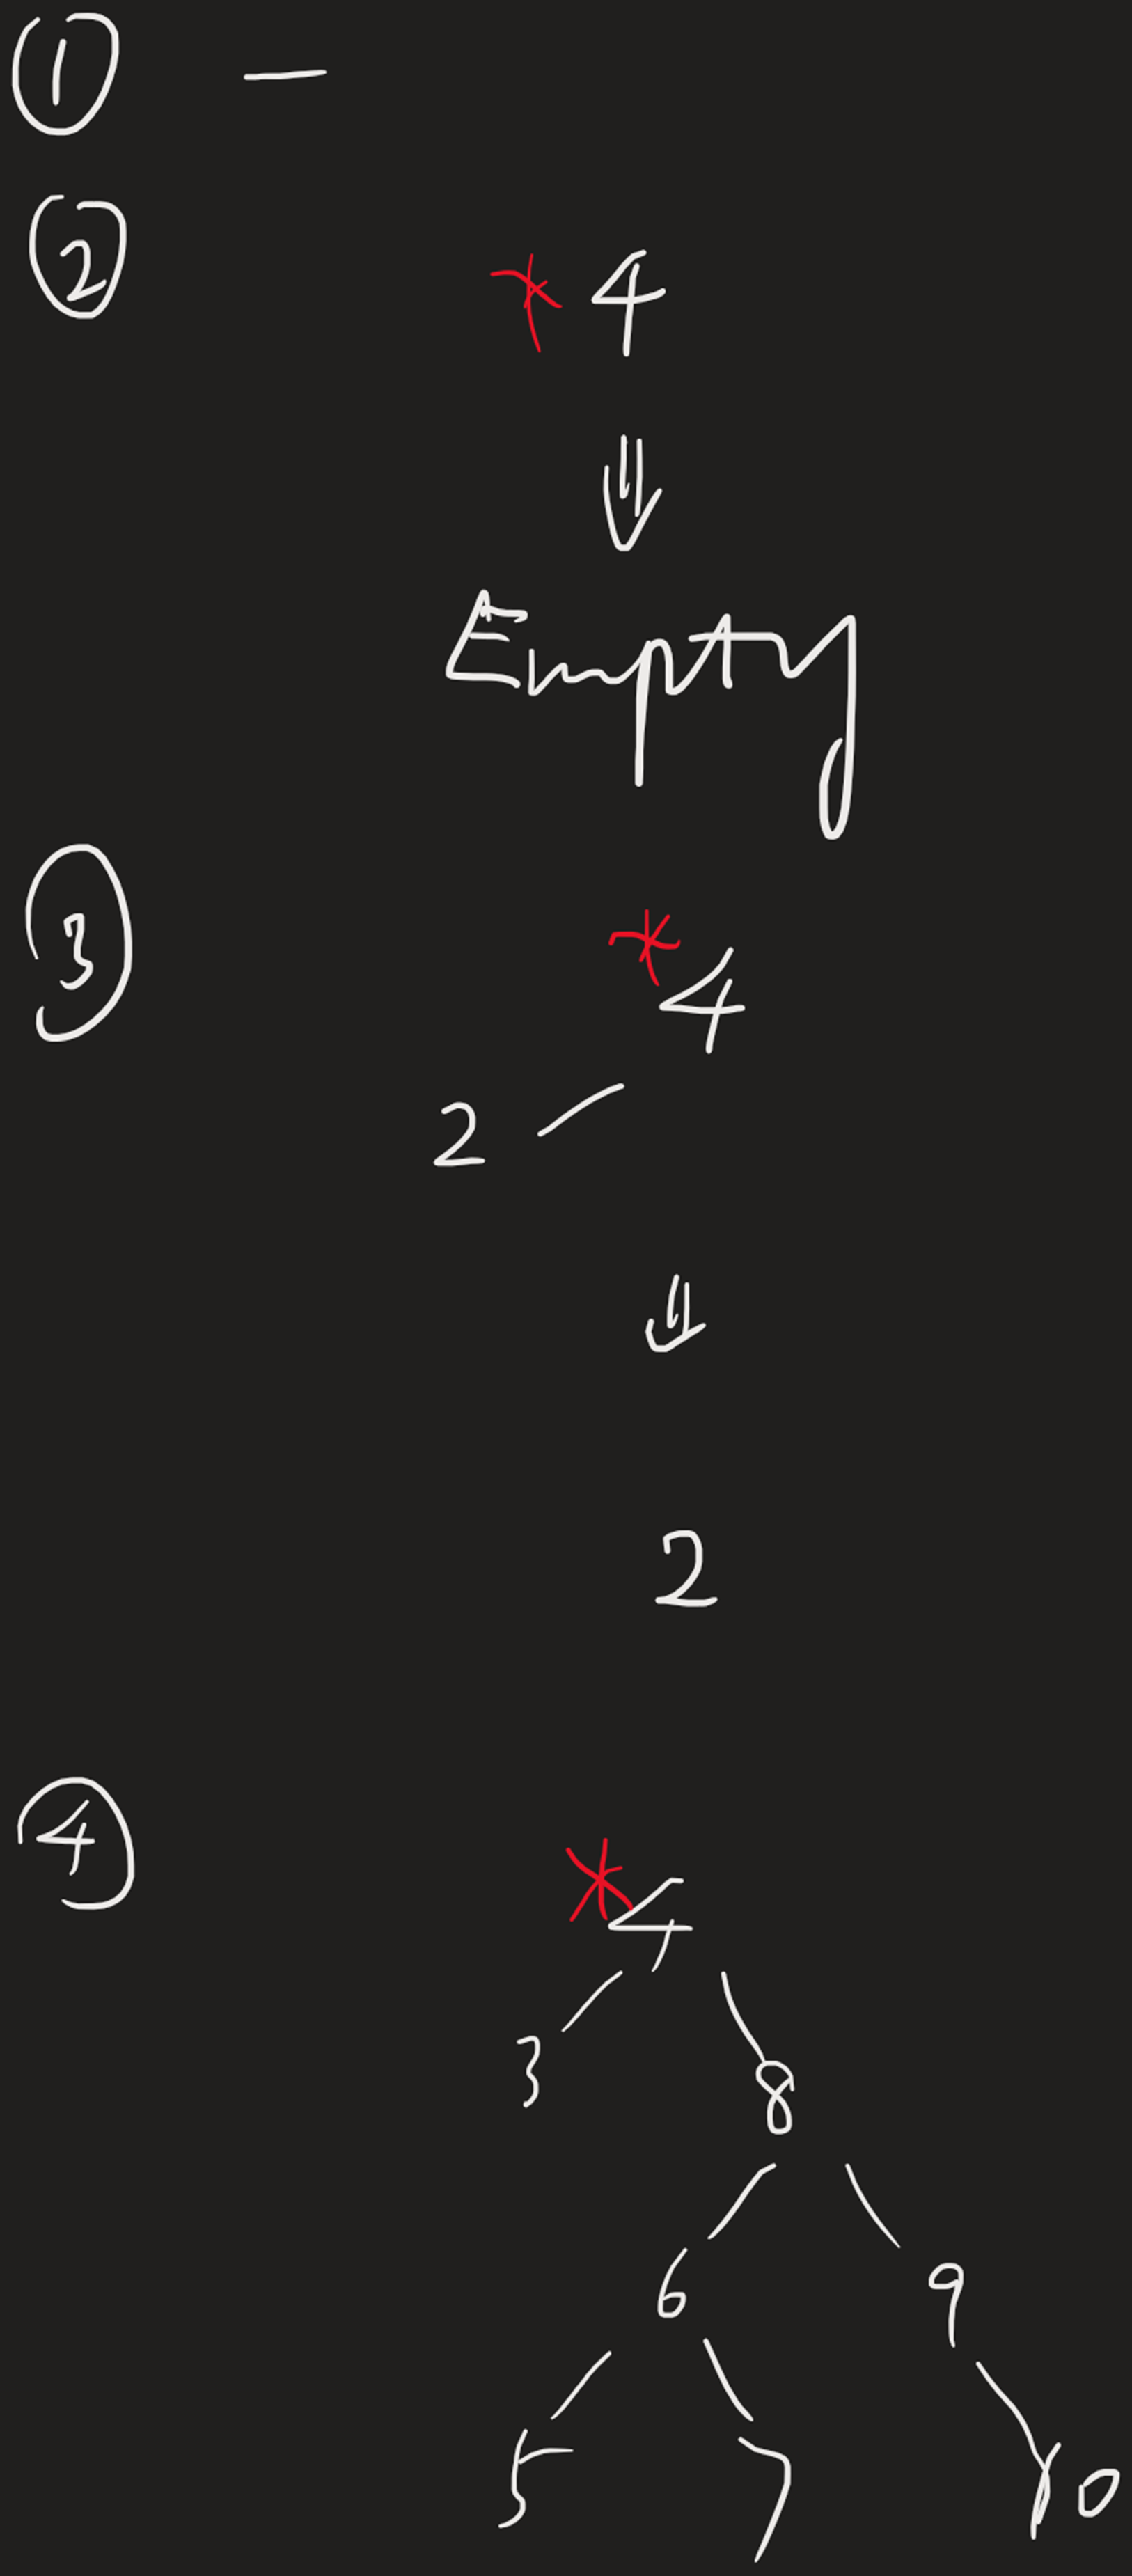
\includegraphics[width=0.6\textwidth]{1.png}

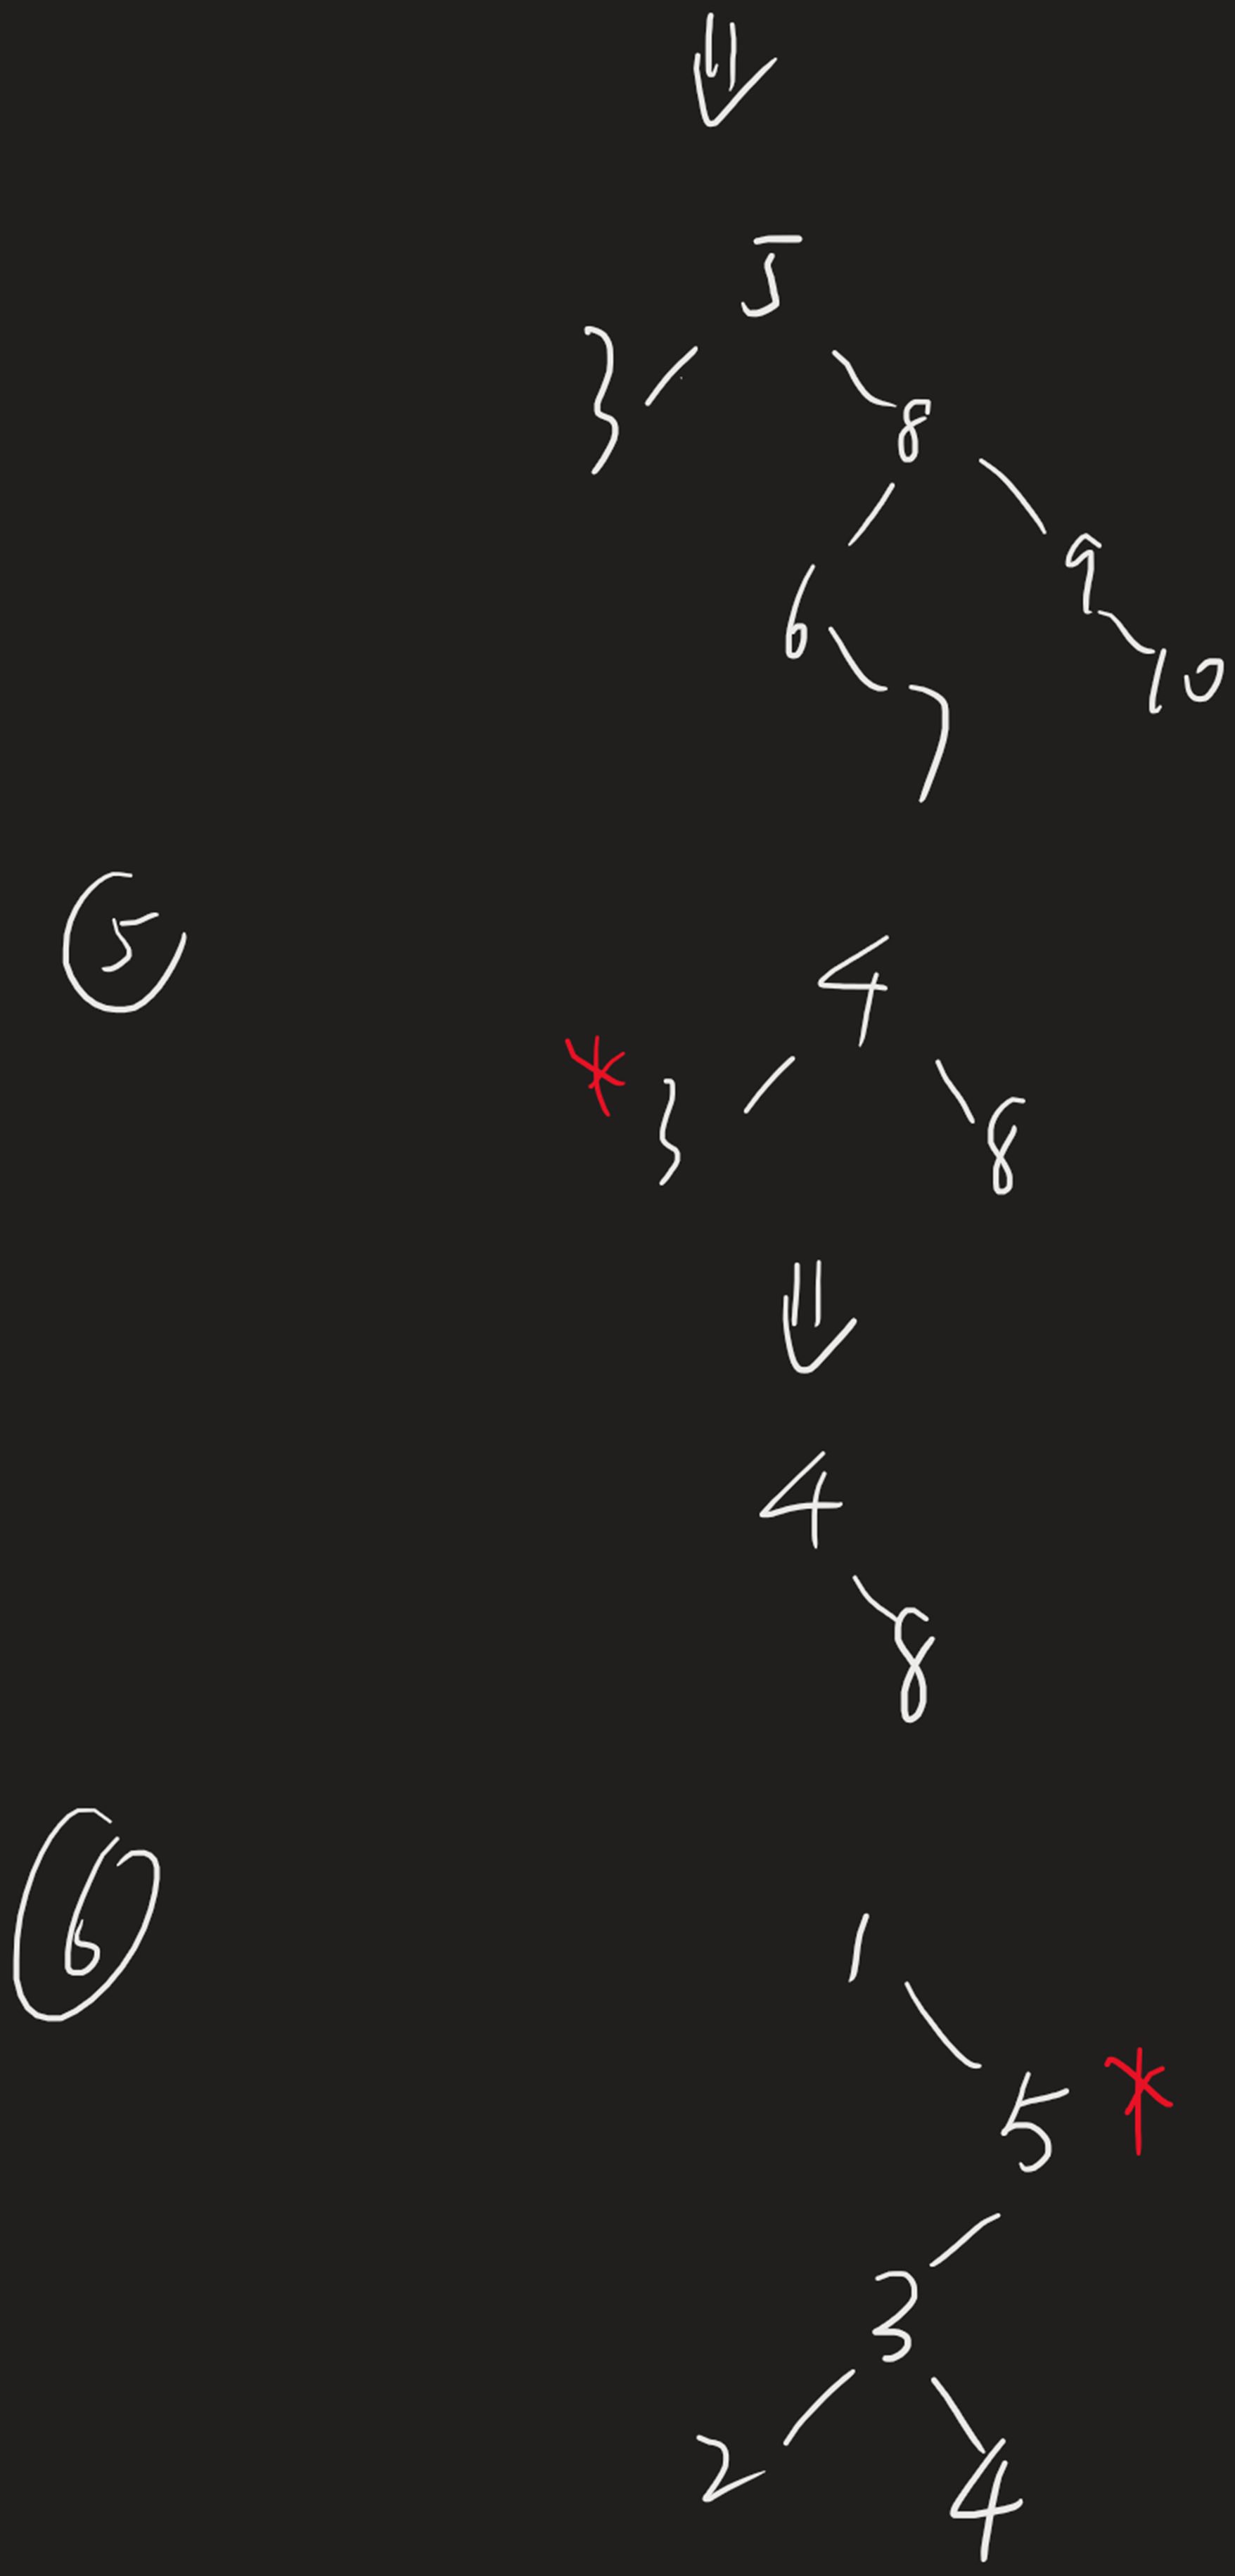
\includegraphics[width=0.6\textwidth]{2.png}

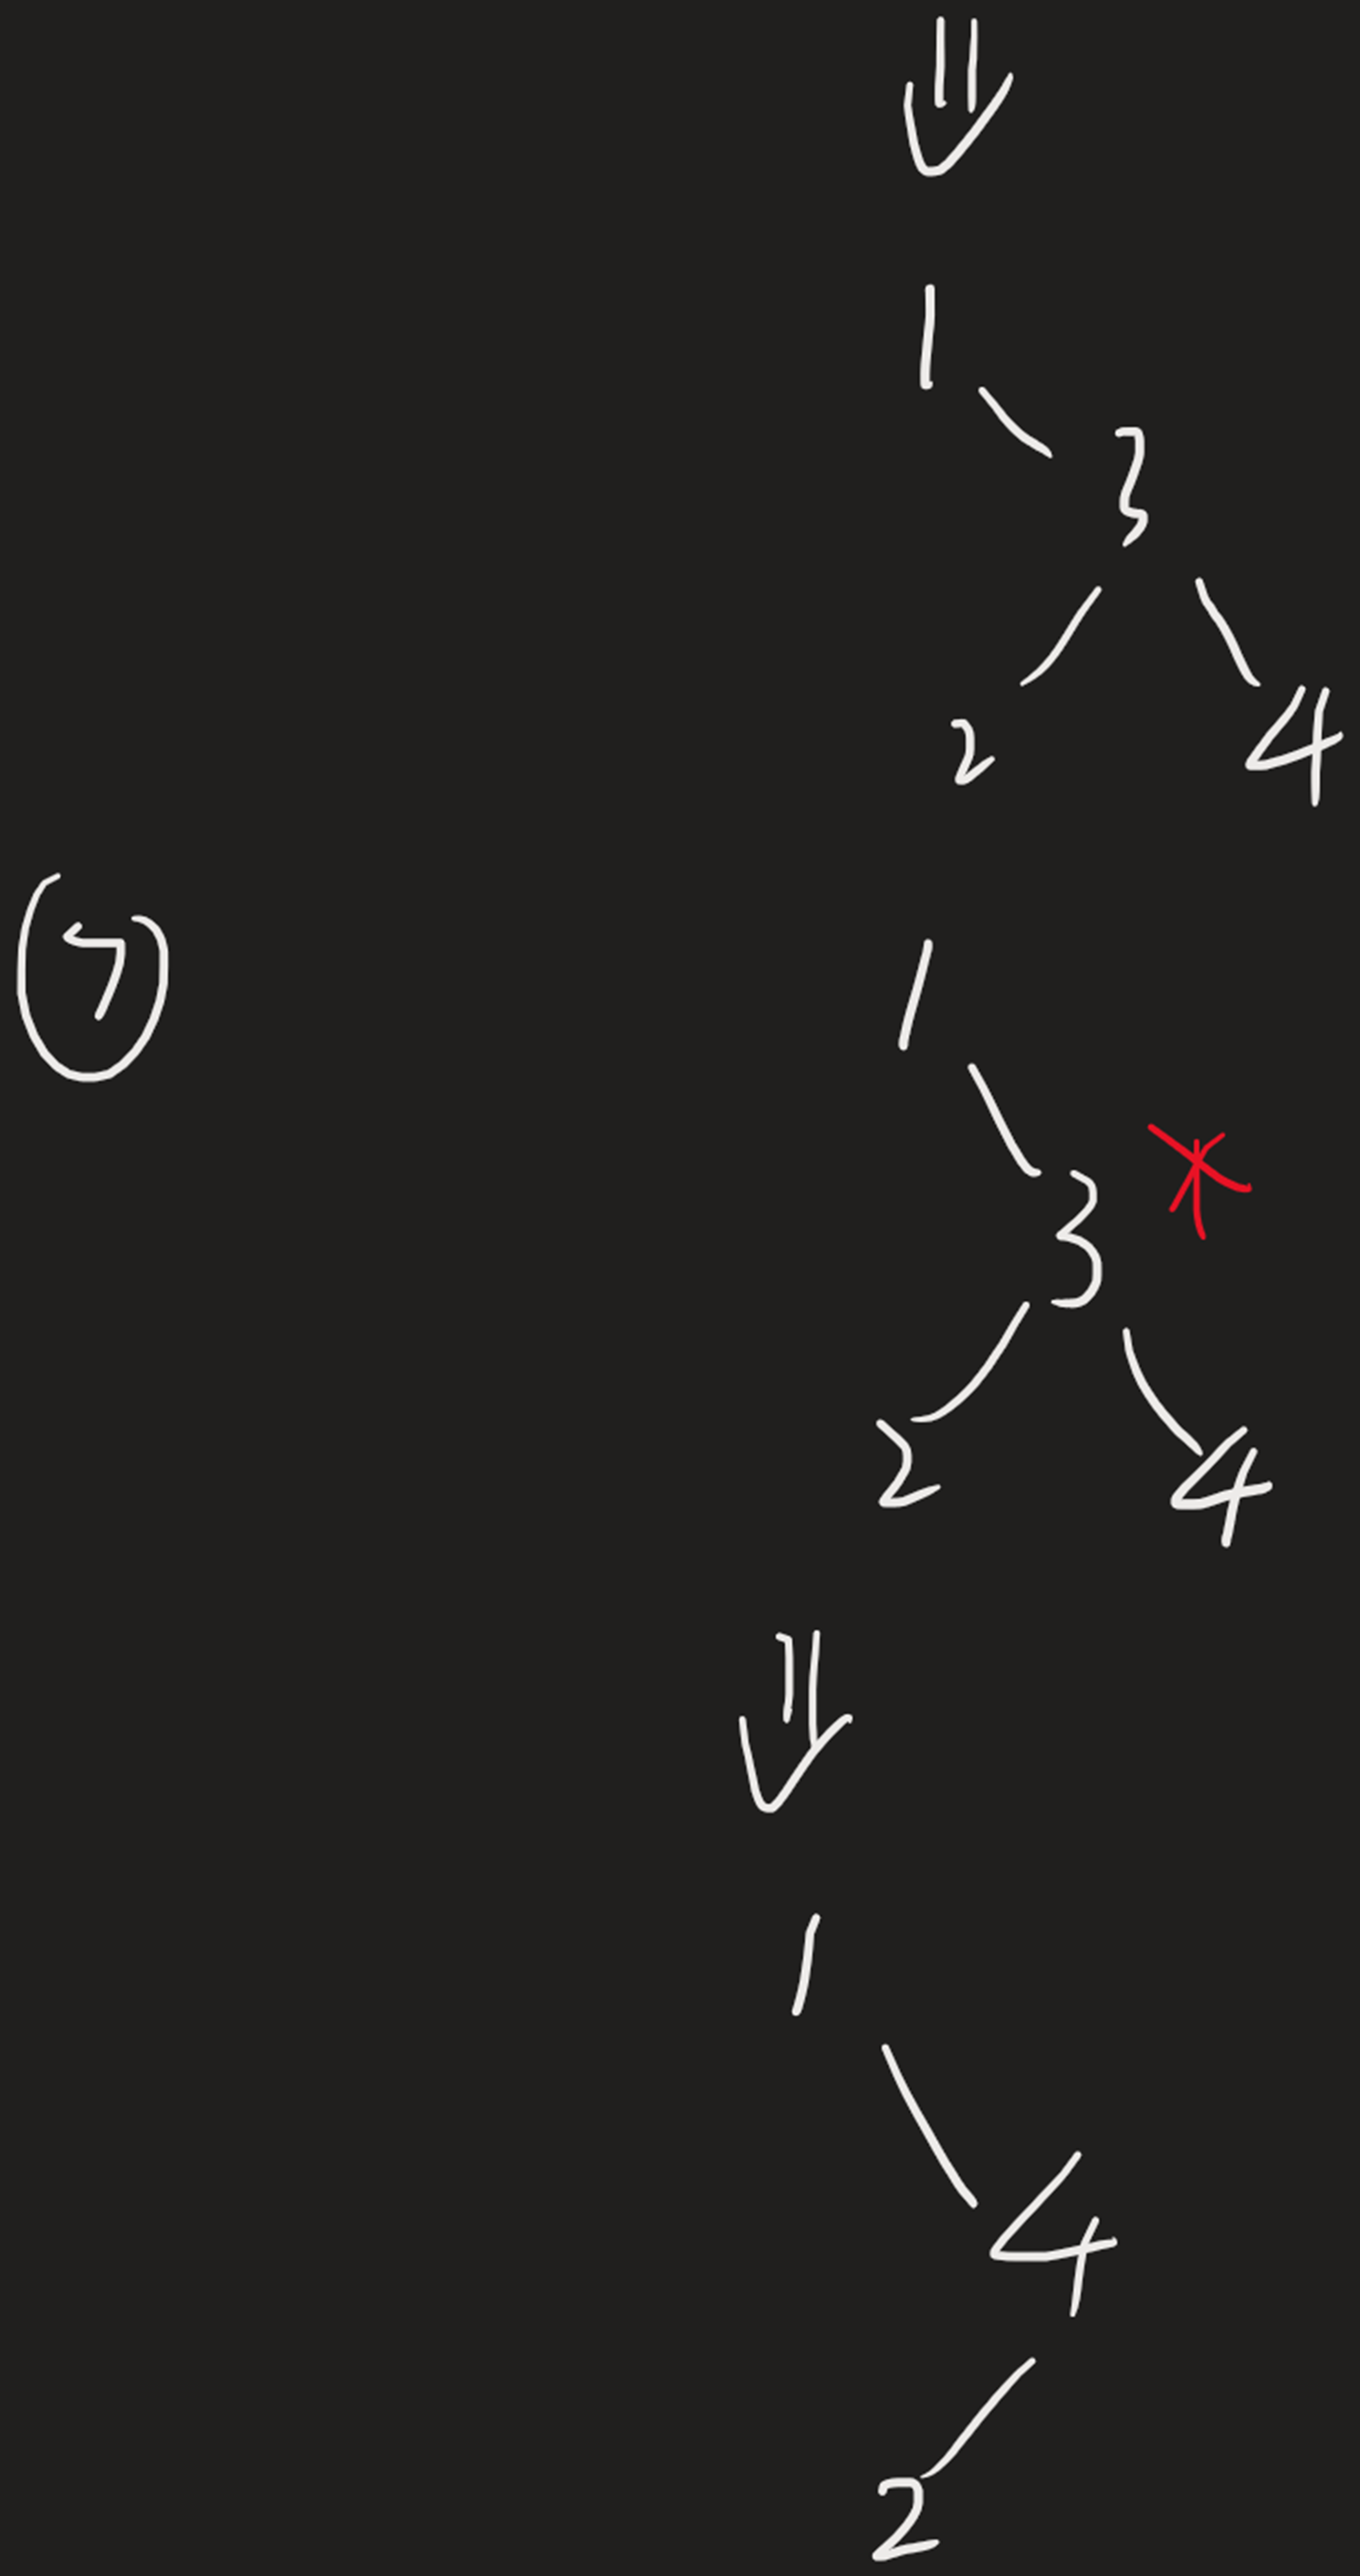
\includegraphics[width=0.6\textwidth]{3.png}

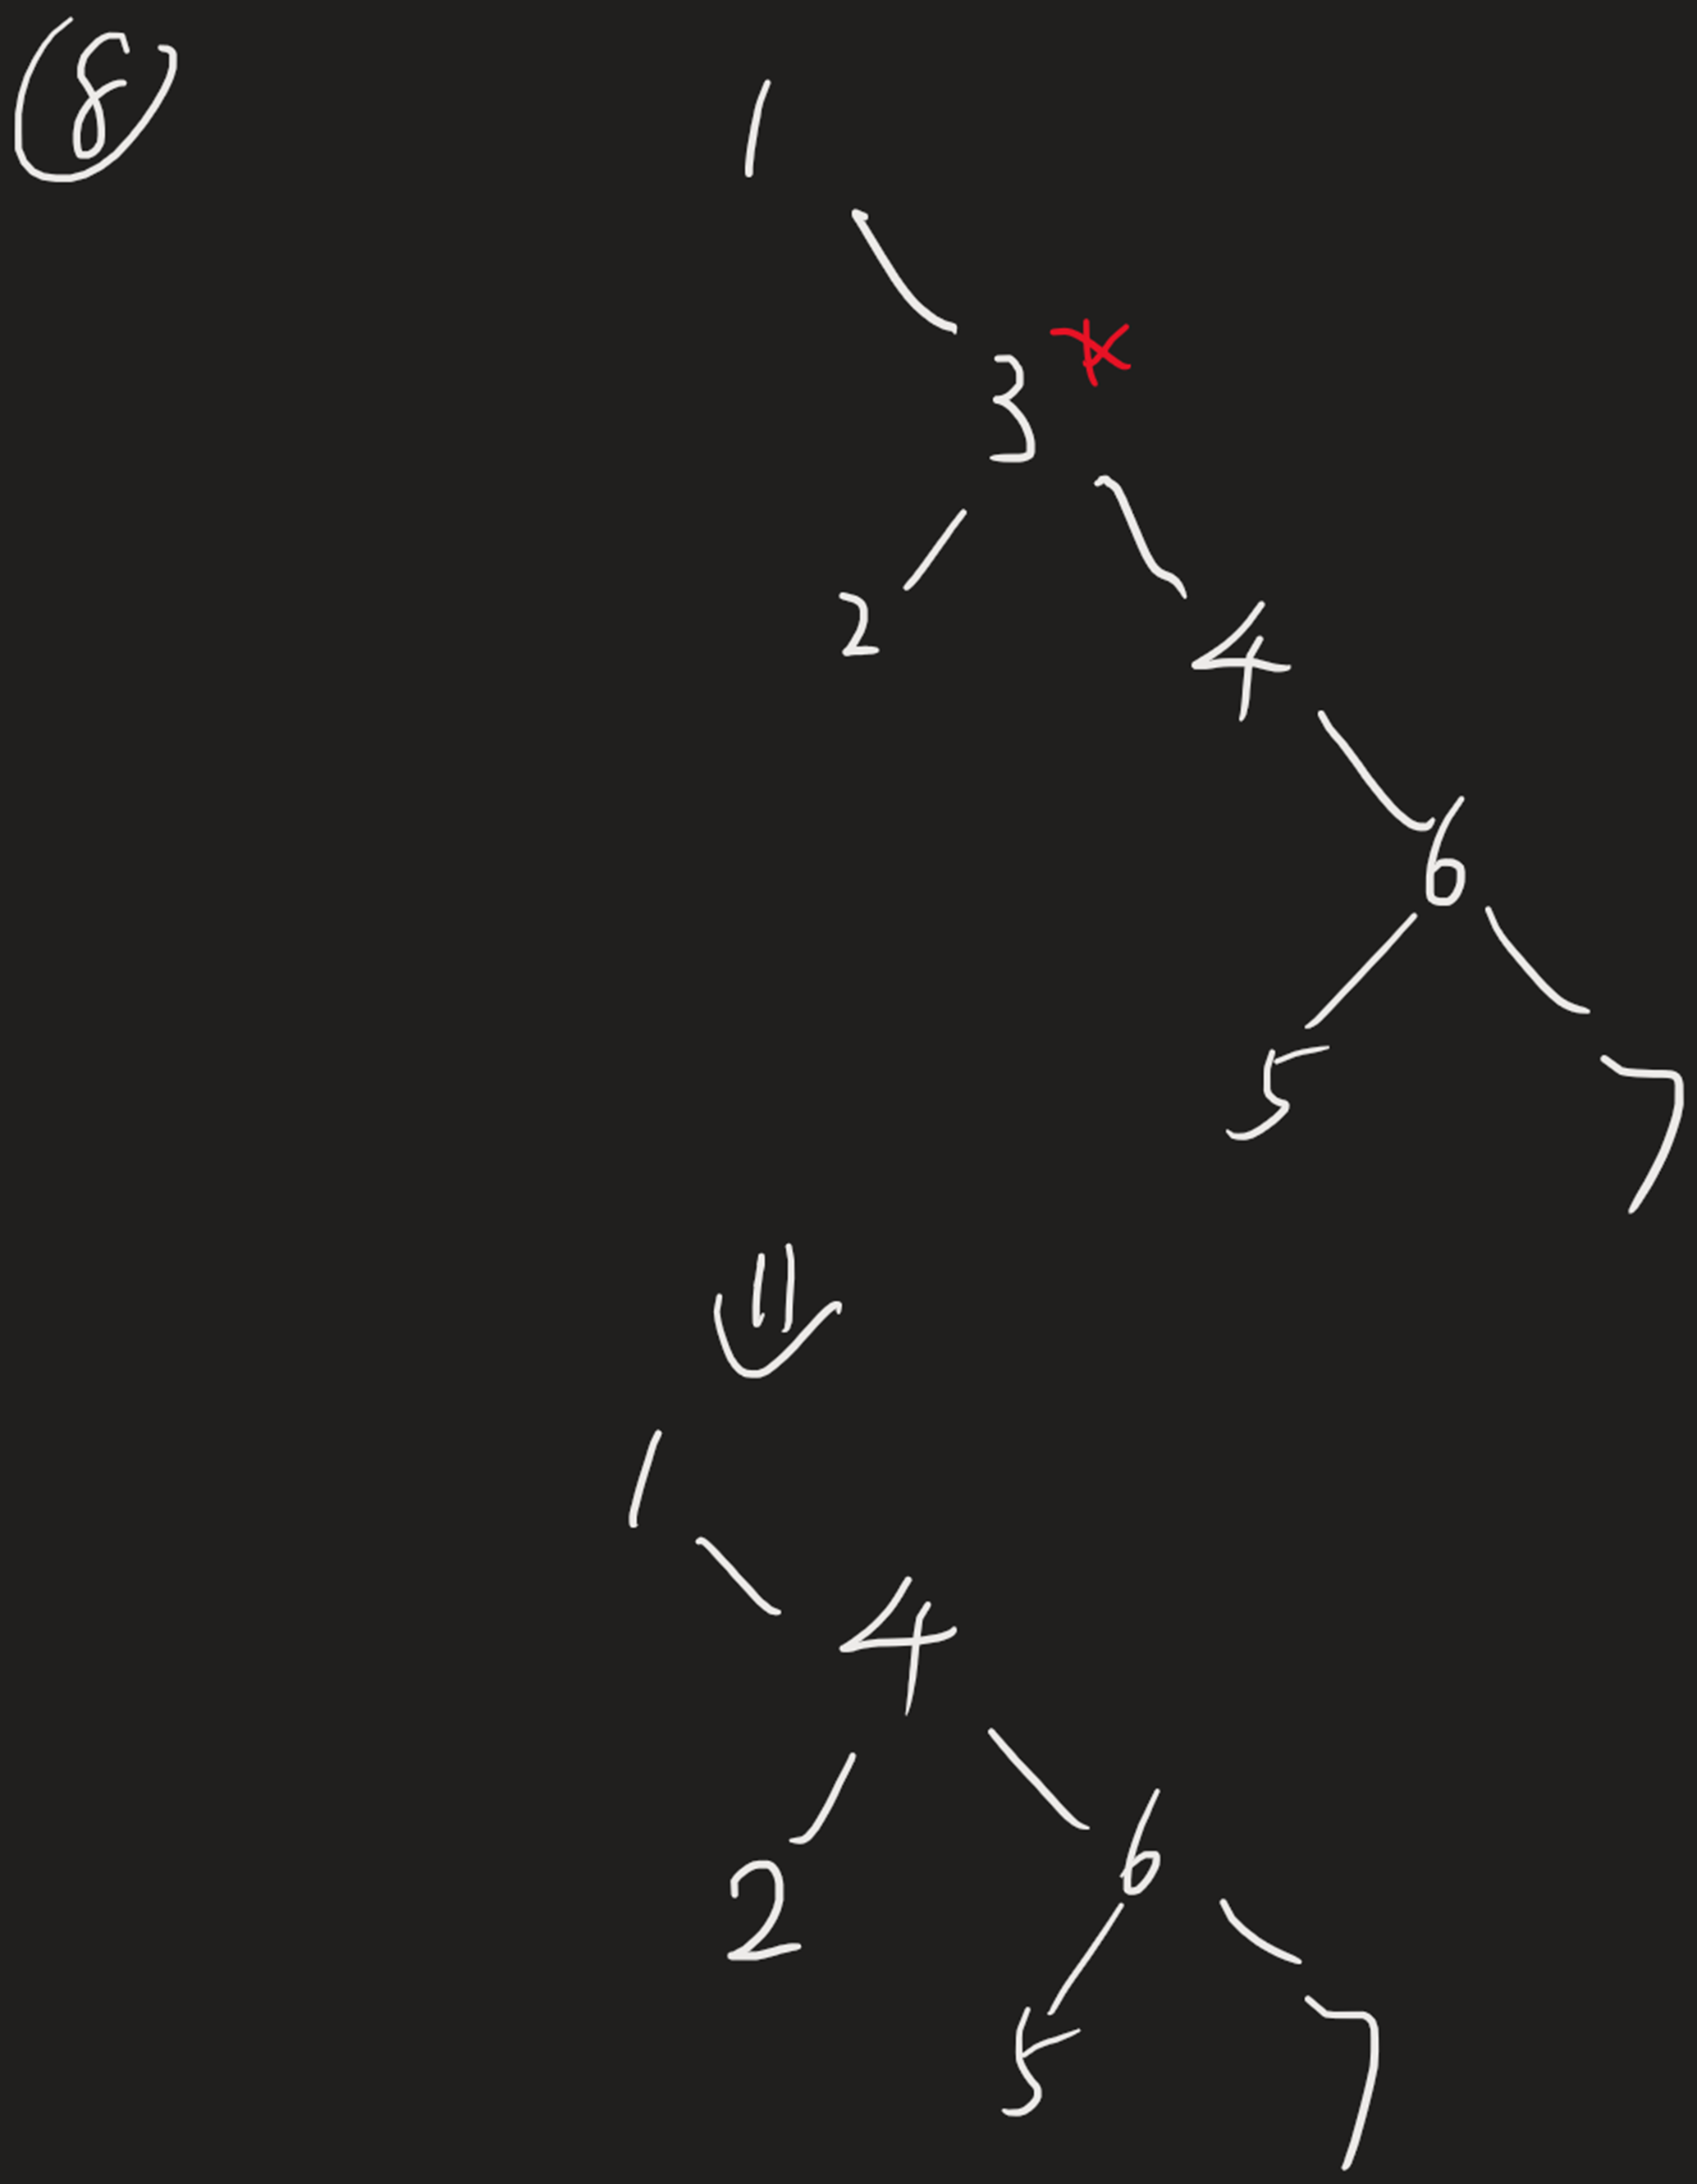
\includegraphics[width=0.6\textwidth]{4.png}

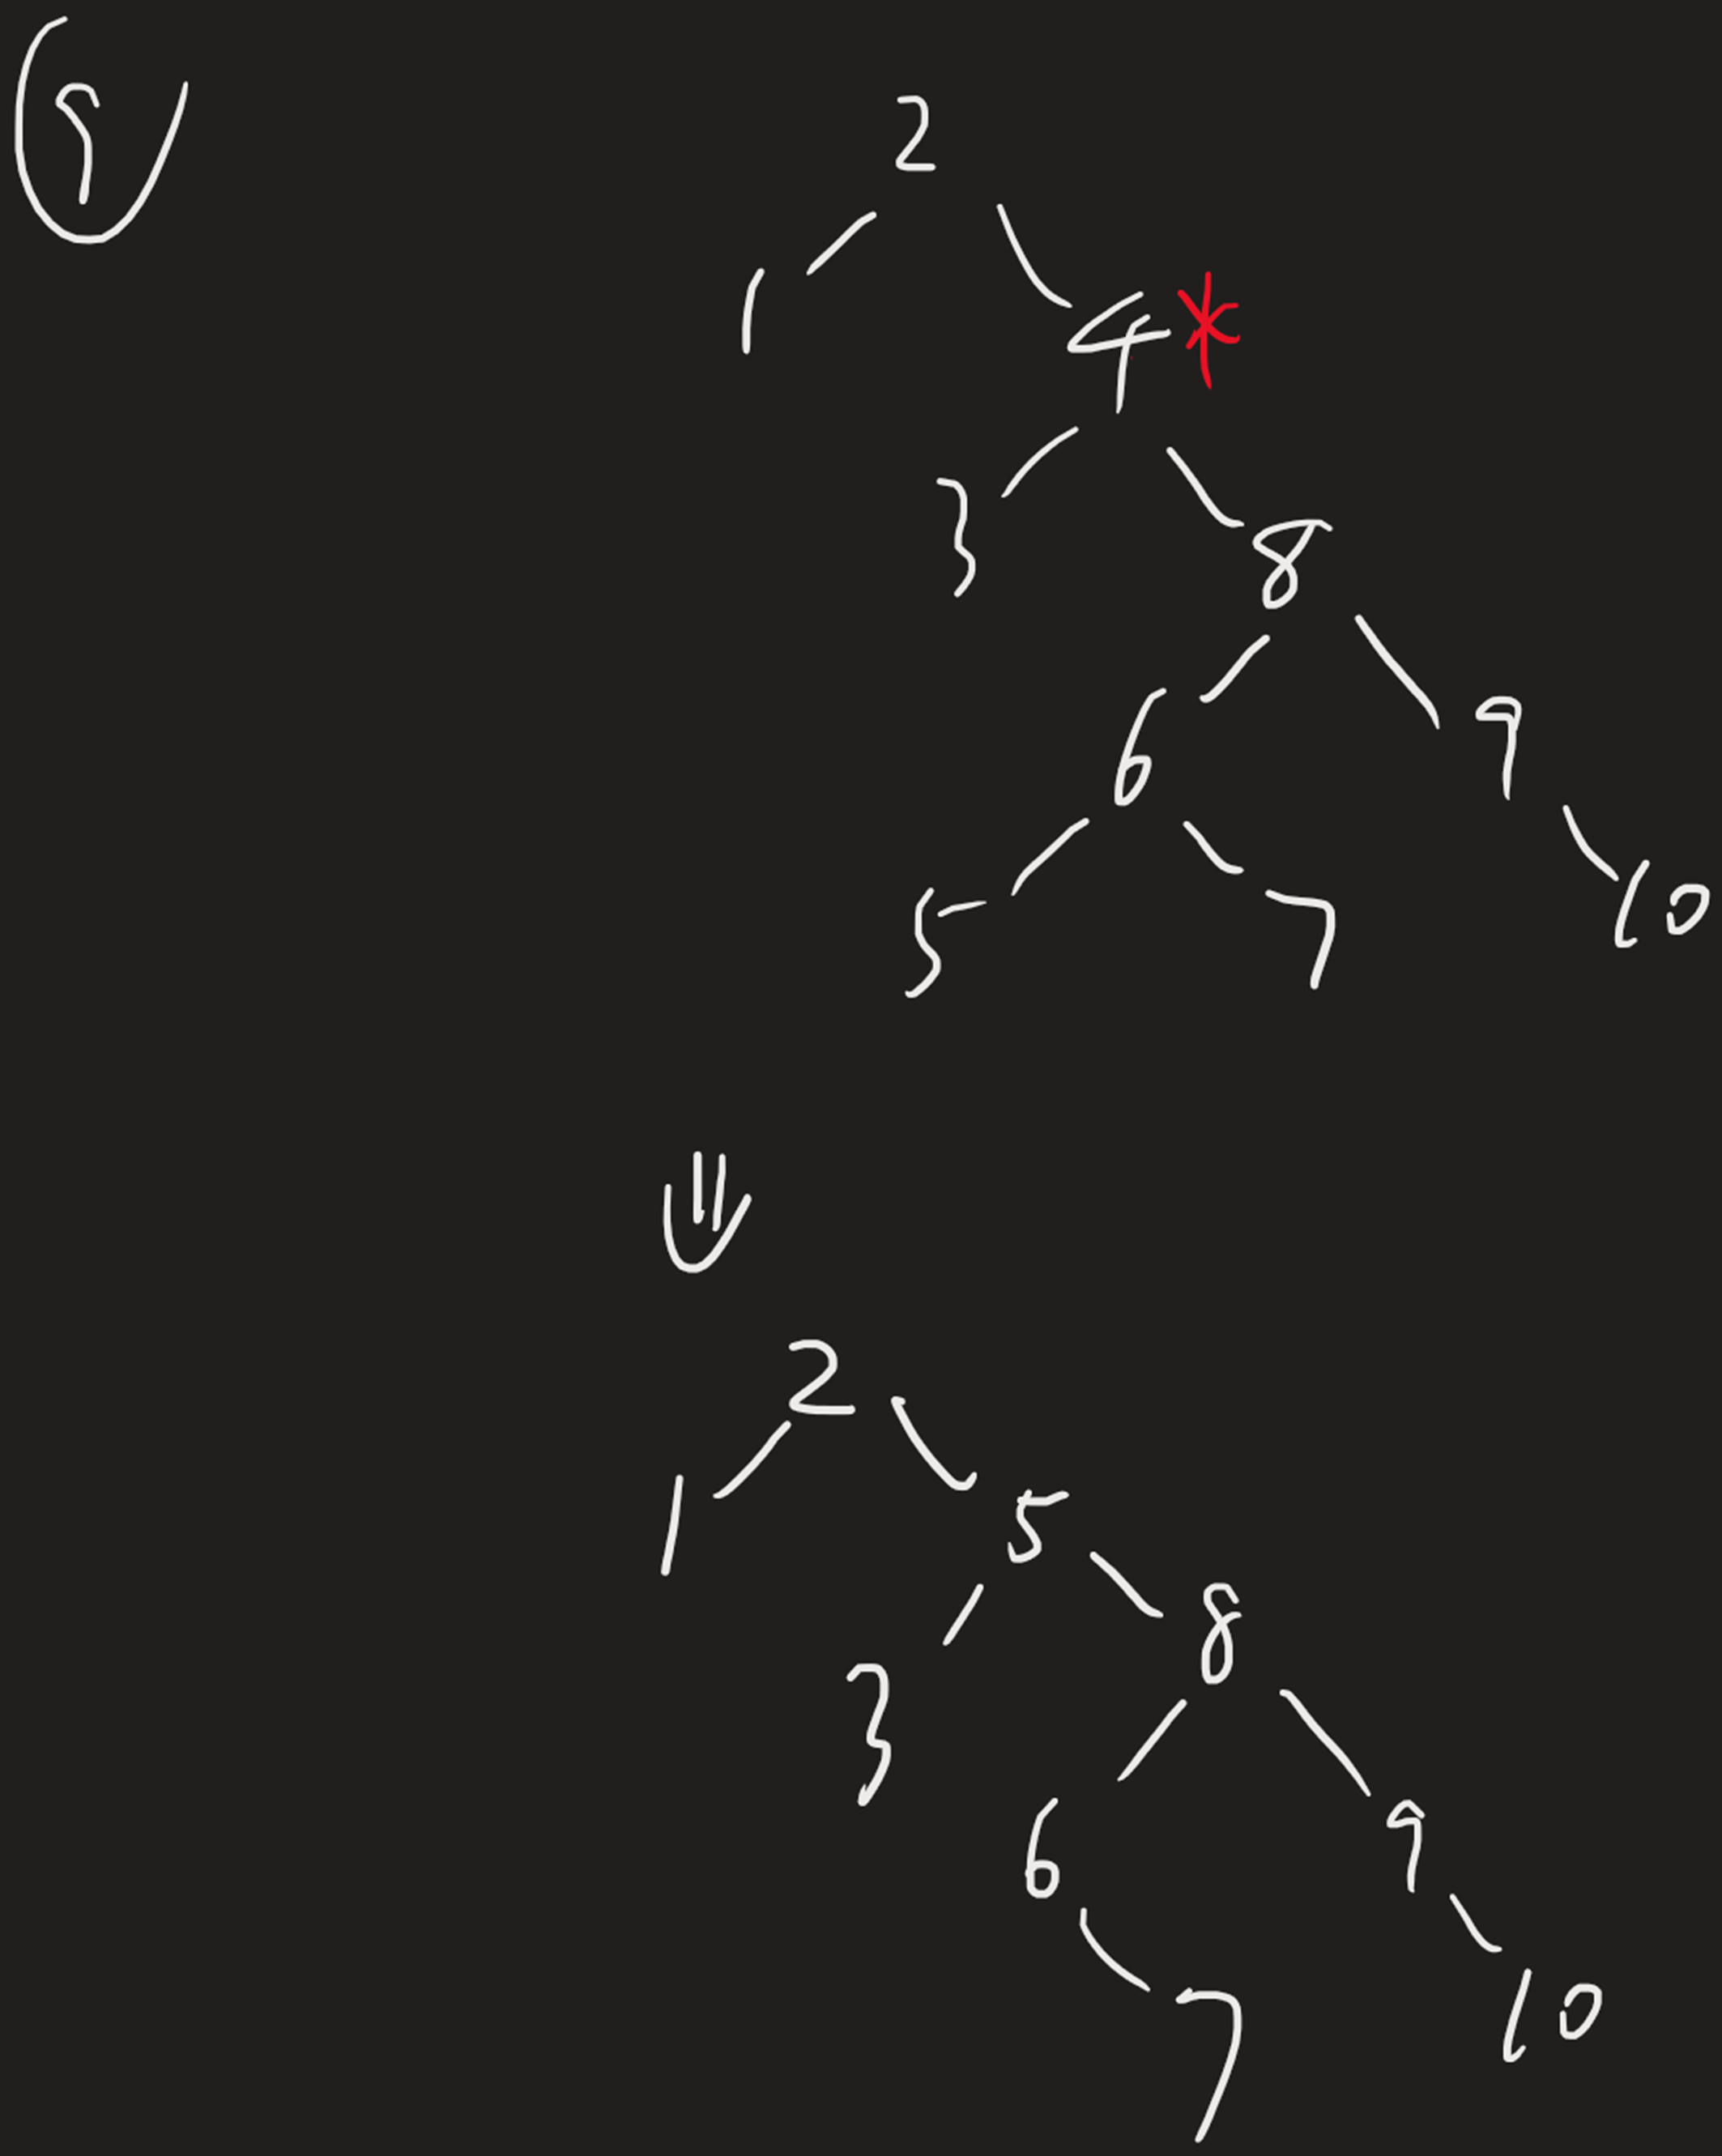
\includegraphics[width=0.6\textwidth]{5.png}

程序输出内容:

\noindent\rule{\textwidth}{1pt}

\begin{verbatim}
1. 找不到要删除的节点:
        删除前的树:
        中序遍历        2       3       5       7       8
        前序遍历        5       3       2       7       8
删除 6
6 is not found.
        删除后的树:
        中序遍历        2       3       5       7       8
        前序遍历        5       3       2       7       8
2. 要删除的节点为根节点,且该节点没有孩子:
        删除前的树:
        中序遍历        4
        前序遍历        4
删除 4
        删除后的树:
Empty tree

Empty tree

3. 要删除的节点为根节点,且该节点只有一个孩子:
        删除前的树:
        中序遍历        2       4
        前序遍历        4       2
删除 4
        删除后的树:
        中序遍历        2
        前序遍历        2
4. 要删除的节点为根节点,且该节点有两个孩子:
        删除前的树:
        中序遍历        3       4       5       6       7       8       9       10
        前序遍历        4       3       8       6       5       7       9       10
删除 4
        删除后的树:
        中序遍历        3       5       6       7       8       9       10
        前序遍历        5       3       8       6       7       9       10
5. 要删除的节点不是根节点,且该节点没有孩子:
        删除前的树:
        中序遍历        3       4       8
        前序遍历        4       3       8
删除 3
        删除后的树:
        中序遍历        4       8
        前序遍历        4       8
6. 要删除的节点不是根节点,且该节点只有一个孩子:
        删除前的树:
        中序遍历        1       2       3       4       5
        前序遍历        1       5       3       2       4
删除 5
        删除后的树:
        中序遍历        1       2       3       4
        前序遍历        1       3       2       4
7. 要删除的节点不是根节点,该节点有两个孩子,且右节点没有孩子:
        删除前的树:
        中序遍历        1       2       3       4
        前序遍历        1       3       2       4
删除 3
        删除后的树:
        中序遍历        1       2       4
        前序遍历        1       4       2
8. 要删除的节点不是根节点,该节点有两个孩子,且右节点只有一个右孩子:
        删除前的树:
        中序遍历        1       2       3       4       5       6       7
        前序遍历        1       3       2       4       6       5       7
删除 3
        删除后的树:
        中序遍历        1       2       4       5       6       7
        前序遍历        1       4       2       6       5       7
9. 要删除的节点不是根节点,该节点有两个孩子,且右节点有两个孩子:
        删除前的树:
        中序遍历        1       2       3       4       5       6       7       8       9       10
        前序遍历        2       1       4       3       8       6       5       7       9       10
删除 4
        删除后的树:
        中序遍历        1       2       3       5       6       7       8       9       10
        前序遍历        2       1       5       3       8       6       7       9       10
10. 对空树执行remove操作
        删除前的树:
Empty tree

Empty tree

terminate called after throwing an instance of 'UnderflowException'
make: *** [Makefile:23: run] 已放弃 (核心已转储)
\end{verbatim}
\noindent\rule{\textwidth}{1pt}

\end{document}

%%% Local Variables: 
%%% mode: latex
%%% TeX-master: t
%%% End: 
